\chapter{Rad s bitovima}

Svi podaci u računalnim programima interno su pohranjeni kao bitovi,
tj. kao brojevi 0 i 1.
Ovo poglavlje razmatra bitovni zapis
cijelih brojeva i pokazuje primjere
kako koristiti bitovne operacije.
Pokazuje se da rad s bitovima ima mnogo primjena
u algoritamskom programiranju.

\section{Bitovni zapis}

\index{bitovni zapis}

U programiranju, $n$-bitni cijeli broj interno je
pohranjen kao binarni broj koji se sastoji od $n$ bitova.
Na primjer, C++ tip \texttt{int} je
32-bitni tip, što znači da se svaki \texttt{int}
broj sastoji od 32 bita.

Evo bitovnog zapisa
\texttt{int} broja 43: 
\[00000000000000000000000000101011\]
Bitovi u zapisu indeksirani su zdesna nalijevo.
Da bismo bitovni zapis $b_k \cdots b_2 b_1 b_0$ pretvorili u broj,
možemo koristiti formulu
\[b_k 2^k + \ldots + b_2 2^2 + b_1 2^1 + b_0 2^0.\]
Na primjer,
\[1 \cdot 2^5 + 1 \cdot 2^3 + 1 \cdot 2^1 + 1 \cdot 2^0 = 43.\]

Bitovni zapis broja je ili
\key{predznačen} ili \key{nepredznačen}.
Obično se koristi predznačeni zapis,
što znači da se mogu prikazati i negativni
i pozitivni brojevi.
Predznačena varijabla od $n$ bitova može sadržavati bilo koji
cijeli broj između $-2^{n-1}$ i $2^{n-1}-1$.
Na primjer, tip \texttt{int} u C++-u je
predznačeni tip, pa \texttt{int} varijabla može sadržavati bilo koji
cijeli broj između $-2^{31}$ i $2^{31}-1$.

Prvi bit u predznačenom zapisu
predznak je broja (0 za nenegativne brojeve,
a 1 za negativne brojeve), dok
preostalih $n-1$ bitova sadrži iznos broja.
Koristi se \key{dvojni komplement}, što znači da se
suprotni broj nekog broja izračunava tako da se prvo
invertiraju svi bitovi u broju,
a zatim se broj uveća za jedan.

Na primjer, bitovni zapis
\texttt{int} broja $-43$ je
\[11111111111111111111111111010101.\]

U nepredznačenom zapisu mogu se koristiti samo nenegativni
brojevi, ali je gornja ograda za vrijednosti veća.
Nepredznačena varijabla od $n$ bitova može sadržavati bilo koji
cijeli broj između $0$ i $2^n-1$.
Na primjer, u C++-u \texttt{unsigned int} varijabla
može sadržavati bilo koji cijeli broj između $0$ i $2^{32}-1$.

Postoji veza između tih
zapisa:
predznačeni broj $-x$ jednak je nepredznačenom broju $2^n-x$.
Na primjer, sljedeći kod pokazuje da je
predznačeni broj $x=-43$ jednak nepredznačenom
broju $y=2^{32}-43$:
\begin{lstlisting}
int x = -43;
unsigned int y = x;
cout << x << "\n"; // -43
cout << y << "\n"; // 4294967253
\end{lstlisting}

Ako je broj veći od gornje ograde
bitovnog zapisa, dolazi do prelijevanja broja.
U predznačenom zapisu
sljedeći broj nakon $2^{n-1}-1$ je $-2^{n-1}$,
a u nepredznačenom zapisu
sljedeći broj nakon $2^n-1$ je $0$.
Na primjer, razmotrimo sljedeći kod:
\begin{lstlisting}
int x = 2147483647
cout << x << "\n"; // 2147483647
x++;
cout << x << "\n"; // -2147483648
\end{lstlisting}

Na početku je vrijednost varijable $x$ jednaka $2^{31}-1$.
To je najveća vrijednost koja se može pohraniti
u \texttt{int} varijablu,
pa je sljedeći broj nakon $2^{31}-1$ broj $-2^{31}$.


\section{Bitovne operacije}

\newcommand\XOR{\mathbin{\char`\^}}

\subsubsection{Operacija and}

\index{operacija and}

Operacija \key{and} $x$ \& $y$ daje broj
koji ima jedinične bitove na pozicijama gdje i
$x$ i $y$ imaju jedinične bitove.
Na primjer, $22$ \& $26$ = 18, jer

\begin{center}
\begin{tabular}{rrr}
& 10110 & (22)\\
\& & 11010 & (26) \\
\hline
 = & 10010 & (18) \\
\end{tabular}
\end{center}

Pomoću operacije and možemo provjeriti je li broj
$x$ paran, jer je
$x$ \& $1$ = 0 ako je $x$ paran, a
$x$ \& $1$ = 1 ako je $x$ neparan.
Općenitije, $x$ je djeljiv s $2^k$
točno onda kada je $x$ \& $(2^k-1)$ = 0.

\subsubsection{Operacija or}

\index{operacija or}

Operacija \key{or} $x$ | $y$ daje broj
koji ima jedinične bitove na pozicijama gdje barem jedan
od brojeva $x$ i $y$ ima jedinične bitove.
Na primjer, $22$ | $26$ = 30, jer

\begin{center}
\begin{tabular}{rrr}
& 10110 & (22)\\
| & 11010 & (26) \\
\hline
 = & 11110 & (30) \\
\end{tabular}
\end{center}

\subsubsection{Operacija xor}

\index{operacija xor}

Operacija \key{xor} $x$ $\XOR$ $y$ daje broj
koji ima jedinične bitove na pozicijama gdje točno jedan
od brojeva $x$ i $y$ ima jedinične bitove.
Na primjer, $22$ $\XOR$ $26$ = 12, jer

\begin{center}
\begin{tabular}{rrr}
& 10110 & (22)\\
$\XOR$ & 11010 & (26) \\
\hline
 = & 01100 & (12) \\
\end{tabular}
\end{center}

\subsubsection{Operacija not}

\index{operacija not}

Operacija \key{not} \textasciitilde$x$
daje broj u kojem su svi bitovi broja $x$
invertirani.
Vrijedi formula \textasciitilde$x = -x-1$,
na primjer, \textasciitilde$29 = -30$.

Rezultat operacije not na razini bitova
ovisi o duljini bitovnog zapisa,
jer operacija invertira sve bitove.
Na primjer, ako su brojevi 32-bitni
\texttt{int} brojevi, rezultat je sljedeći:

\begin{center}
\begin{tabular}{rrrr}
$x$ & = & 29 &   00000000000000000000000000011101 \\
\textasciitilde$x$ & = & $-30$ & 11111111111111111111111111100010 \\
\end{tabular}
\end{center}

\subsubsection{Bitovni pomaci}

\index{bitovni pomak}

Lijevi bitovni pomak $x < < k$ dodaje $k$
nul-bitova na kraj broja,
a desni bitovni pomak $x > > k$
uklanja $k$ posljednjih bitova iz broja.
Na primjer, $14 < < 2 = 56$,
jer $14$ i $56$ odgovaraju zapisima 1110 i 111000.
Slično, $49 > > 3 = 6$,
jer $49$ i $6$ odgovaraju zapisima 110001 i 110.

Uočimo da $x < < k$
odgovara množenju broja $x$ s $2^k$,
a $x > > k$
odgovara dijeljenju broja $x$ s $2^k$
zaokruženom naniže na cijeli broj.

\subsubsection{Primjene}

Broj oblika $1 < < k$ ima jedinični bit
na poziciji $k$, a svi ostali bitovi su nula,
pa takve brojeve možemo koristiti za pristup pojedinim bitovima brojeva.
Konkretno, $k$-ti bit broja jednak je jedan
točno onda kada $x$ \& $(1 < < k)$ nije nula.
Sljedeći kod ispisuje bitovni zapis
\texttt{int} broja $x$:

\begin{lstlisting}
for (int i = 31; i >= 0; i--) {
    if (x&(1<<i)) cout << "1";
    else cout << "0";
}
\end{lstlisting}

Sličnim idejama moguće je i mijenjati pojedine bitove
brojeva.
Na primjer, formula $x$ | $(1 < < k)$
postavlja $k$-ti bit broja $x$ na jedan,
formula
$x$ \& \textasciitilde $(1 < < k)$
postavlja $k$-ti bit broja $x$ na nulu,
a formula
$x$ $\XOR$ $(1 < < k)$
invertira $k$-ti bit broja $x$.

Formula $x$ \& $(x-1)$ postavlja posljednji
jedinični bit broja $x$ na nulu,
a formula $x$ \& $-x$ postavlja sve
jedinične bitove na nulu, osim posljednjeg jediničnog bita.
Formula $x$ | $(x-1)$
invertira sve bitove nakon posljednjeg jediničnog bita.
Također uočimo da je pozitivan broj $x$
potencija broja dva točno onda kada je $x$ \& $(x-1) = 0$.

\subsubsection*{Dodatne funkcije}

Prevoditelj (compiler) g++ pruža sljedeće
funkcije za brojanje bitova:

\begin{itemize}
\item
$\texttt{\_\_builtin\_clz}(x)$:
broj nula na početku broja
\item
$\texttt{\_\_builtin\_ctz}(x)$:
broj nula na kraju broja
\item
$\texttt{\_\_builtin\_popcount}(x)$:
broj jedinica u broju
\item
$\texttt{\_\_builtin\_parity}(x)$:
parnost (parna ili neparna) broja jedinica
\end{itemize}
\begin{samepage}

Funkcije se mogu koristiti ovako:
\begin{lstlisting}
int x = 5328; // 00000000000000000001010011010000
cout << __builtin_clz(x) << "\n"; // 19
cout << __builtin_ctz(x) << "\n"; // 4
cout << __builtin_popcount(x) << "\n"; // 5
cout << __builtin_parity(x) << "\n"; // 1
\end{lstlisting}
\end{samepage}

Iako navedene funkcije podržavaju samo \texttt{int} brojeve,
dostupne su i \texttt{long long} verzije
tih funkcija sa sufiksom \texttt{ll}.

\section{Prikaz skupova}

Svaki podskup skupa
$\{0,1,2,\ldots,n-1\}$
može se prikazati kao $n$-bitni cijeli broj
čiji jedinični bitovi označavaju koji
elementi pripadaju podskupu.
To je efikasan način prikaza skupova,
jer svaki element zahtijeva samo jedan bit memorije,
a operacije nad skupovima mogu se implementirati kao bitovne operacije.

Na primjer, budući da je \texttt{int} 32-bitni tip,
\texttt{int} broj može prikazati bilo koji podskup
skupa $\{0,1,2,\ldots,31\}$.
Bitovni zapis skupa $\{1,3,4,8\}$ je
\[00000000000000000000000100011010,\]
što odgovara broju $2^8+2^4+2^3+2^1=282$.

\subsubsection{Implementacija skupa}

Sljedeći kod deklarira \texttt{int}
varijablu $x$ koja može sadržavati
podskup skupa $\{0,1,2,\ldots,31\}$.
Nakon toga kod dodaje elemente 1, 3, 4 i 8
u skup i ispisuje veličinu skupa.
\begin{lstlisting}
int x = 0;
x |= (1<<1);
x |= (1<<3);
x |= (1<<4);
x |= (1<<8);
cout << __builtin_popcount(x) << "\n"; // 4
\end{lstlisting}
Zatim, sljedeći kod ispisuje sve
elemente koji pripadaju skupu:
\begin{lstlisting}
for (int i = 0; i < 32; i++) {
    if (x&(1<<i)) cout << i << " ";
}
// output: 1 3 4 8
\end{lstlisting}

\subsubsection{Operacije nad skupovima}

Operacije nad skupovima mogu se implementirati kao bitovne operacije na sljedeći način:

\begin{center}
\begin{tabular}{lll}
& skupovna sintaksa & bitovna sintaksa \\
\hline
presjek & $a \cap b$ & $a$ \& $b$ \\
unija & $a \cup b$ & $a$ | $b$ \\
komplement & $\bar a$ & \textasciitilde$a$ \\
razlika & $a \setminus b$ & $a$ \& (\textasciitilde$b$) \\
\end{tabular}
\end{center}

Na primjer, sljedeći kod najprije konstruira
skupove $x=\{1,3,4,8\}$ i $y=\{3,6,8,9\}$,
a zatim konstruira skup $z = x \cup y = \{1,3,4,6,8,9\}$:

\begin{lstlisting}
int x = (1<<1)|(1<<3)|(1<<4)|(1<<8);
int y = (1<<3)|(1<<6)|(1<<8)|(1<<9);
int z = x|y;
cout << __builtin_popcount(z) << "\n"; // 6
\end{lstlisting}

\subsubsection{Prolazak kroz podskupove}

Sljedeći kod prolazi kroz
podskupove skupa $\{0,1,\ldots,n-1\}$:

\begin{lstlisting}
for (int b = 0; b < (1<<n); b++) {
    // process subset b
}
\end{lstlisting}
Sljedeći kod prolazi kroz
podskupove s točno $k$ elemenata:
\begin{lstlisting}
for (int b = 0; b < (1<<n); b++) {
    if (__builtin_popcount(b) == k) {
        // process subset b
    }
}
\end{lstlisting}
Sljedeći kod prolazi kroz podskupove
skupa $x$:
\begin{lstlisting}
int b = 0;
do {
    // process subset b
} while (b=(b-x)&x);
\end{lstlisting}

\section{Bitovne optimizacije}

Mnogi se algoritmi mogu optimizirati pomoću
bitovnih operacija.
Takve optimizacije ne mijenjaju
vremensku složenost algoritma,
ali mogu imati velik utjecaj
na stvarno vrijeme izvođenja koda.
U ovom odjeljku razmatramo primjere
takvih situacija.

\subsubsection{Hammingove udaljenosti}

\index{Hammingova udaljenost}
\key{Hammingova udaljenost}
$\texttt{hamming}(a,b)$ između dvaju
znakovnih nizova $a$ i $b$ jednake duljine jest
broj pozicija na kojima se nizovi razlikuju.
Na primjer,
\[\texttt{hamming}(01101,11001)=2.\]

Razmotrimo sljedeći zadatak: Zadana je
lista od $n$ bitovnih nizova, svaki duljine $k$;
izračunajte minimalnu Hammingovu udaljenost
između dvaju nizova u listi.
Na primjer, odgovor za $[00111,01101,11110]$
je 2, jer
\begin{itemize}[noitemsep]
\item $\texttt{hamming}(00111,01101)=2$,
\item $\texttt{hamming}(00111,11110)=3$, i
\item $\texttt{hamming}(01101,11110)=3$.
\end{itemize}

Izravan način rješavanja zadatka jest
proći kroz sve parove nizova i izračunati
njihove Hammingove udaljenosti,
što daje algoritam vremenske složenosti $O(n^2 k)$.
Sljedeća funkcija može se koristiti za
računanje udaljenosti:
\begin{lstlisting}
int hamming(string a, string b) {
    int d = 0;
    for (int i = 0; i < k; i++) {
        if (a[i] != b[i]) d++;
    }
    return d;
}
\end{lstlisting}

Međutim, ako je $k$ malen, kod možemo optimizirati
tako da bitovne nizove pohranimo kao cijele brojeve i
Hammingove udaljenosti računamo bitovnim operacijama.
Konkretno, ako je $k \le 32$, nizove možemo jednostavno pohraniti
kao \texttt{int} vrijednosti i koristiti
sljedeću funkciju za računanje udaljenosti:
\begin{lstlisting}
int hamming(int a, int b) {
    return __builtin_popcount(a^b);
}
\end{lstlisting}
U gornjoj funkciji operacija xor konstruira
bitovni niz koji ima jedinične bitove na pozicijama
gdje se $a$ i $b$ razlikuju.
Zatim se broj bitova izračunava pomoću
funkcije \texttt{\_\_builtin\_popcount}.

Da bismo usporedili implementacije, generirali smo
listu od 10000 slučajnih bitovnih nizova duljine 30.
Prvim pristupom pretraga je trajala
13.5 sekundi, a nakon bitovne optimizacije
samo 0.5 sekundi.
Dakle, bitovno optimizirani kod bio je gotovo
30 puta brži od izvornog koda.

\subsubsection{Brojanje podmreža}

Kao drugi primjer, razmotrimo
sljedeći zadatak:
Zadana je mreža veličine $n \times n$ čiji je
svaki kvadrat ili crn (1) ili bijel (0);
izračunajte broj podmreža
čiji su svi kutovi crni.
Na primjer, mreža
\begin{center}
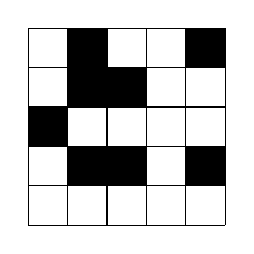
\begin{tikzpicture}[scale=0.5]
\fill[black] (1,1) rectangle (2,2);
\fill[black] (1,4) rectangle (2,5);
\fill[black] (4,1) rectangle (5,2);
\fill[black] (4,4) rectangle (5,5);
\fill[black] (1,3) rectangle (2,4);
\fill[black] (2,3) rectangle (3,4);
\fill[black] (2,1) rectangle (3,2);
\fill[black] (0,2) rectangle (1,3);
\draw (0,0) grid (5,5);
\end{tikzpicture}
\end{center}
sadrži dvije takve podmreže:
\begin{center}
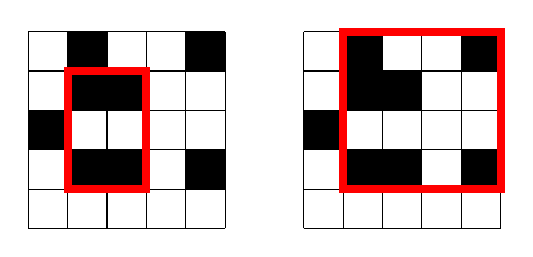
\begin{tikzpicture}[scale=0.5]
\fill[black] (1,1) rectangle (2,2);
\fill[black] (1,4) rectangle (2,5);
\fill[black] (4,1) rectangle (5,2);
\fill[black] (4,4) rectangle (5,5);
\fill[black] (1,3) rectangle (2,4);
\fill[black] (2,3) rectangle (3,4);
\fill[black] (2,1) rectangle (3,2);
\fill[black] (0,2) rectangle (1,3);
\draw (0,0) grid (5,5);

\fill[black] (7+1,1) rectangle (7+2,2);
\fill[black] (7+1,4) rectangle (7+2,5);
\fill[black] (7+4,1) rectangle (7+5,2);
\fill[black] (7+4,4) rectangle (7+5,5);
\fill[black] (7+1,3) rectangle (7+2,4);
\fill[black] (7+2,3) rectangle (7+3,4);
\fill[black] (7+2,1) rectangle (7+3,2);
\fill[black] (7+0,2) rectangle (7+1,3);
\draw (7+0,0) grid (7+5,5);

\draw[color=red,line width=1mm] (1,1) rectangle (3,4);
\draw[color=red,line width=1mm] (7+1,1) rectangle (7+5,5);
\end{tikzpicture}
\end{center}

Postoji algoritam vremenske složenosti $O(n^3)$ za rješavanje zadatka:
prođimo kroz svih $O(n^2)$ parova redaka i za svaki par
$(a,b)$ izračunajmo broj stupaca koji sadrže crni
kvadrat u oba retka u $O(n)$ vremenu.
Sljedeći kod pretpostavlja da $\texttt{color}[y][x]$
označava boju u retku $y$ i stupcu $x$:
\begin{lstlisting}
int count = 0;
for (int i = 0; i < n; i++) {
    if (color[a][i] == 1 && color[b][i] == 1) count++;
}
\end{lstlisting}
Zatim, ti stupci
daju $\texttt{count}(\texttt{count}-1)/2$ podmreža s crnim kutovima,
jer možemo odabrati bilo koja dva od njih da tvore podmrežu.

Da bismo optimizirali ovaj algoritam, mrežu dijelimo na blokove
stupaca tako da se svaki blok sastoji od $N$
uzastopnih stupaca. Tada se svaki redak pohranjuje kao
lista $N$-bitnih brojeva koji opisuju boje
kvadrata. Sada možemo obraditi $N$ stupaca istodobno
pomoću bitovnih operacija. U sljedećem kodu
$\texttt{color}[y][k]$ predstavlja
blok od $N$ boja kao bitove.
\begin{lstlisting}
int count = 0;
for (int i = 0; i <= n/N; i++) {
    count += __builtin_popcount(color[a][i]&color[b][i]);
}
\end{lstlisting}
Dobiveni algoritam radi u $O(n^3/N)$ vremenu.

Generirali smo slučajnu mrežu veličine $2500 \times 2500$
i usporedili izvornu i bitovno optimiziranu implementaciju.
Dok je izvorni kod trajao $29.6$ sekundi,
bitovno optimizirana verzija trajala je samo $3.1$ sekundu
uz $N=32$ (\texttt{int} brojevi) i $1.7$ sekundi
uz $N=64$ (\texttt{long long} brojevi).

\section{Dinamičko programiranje}

Bitovne operacije pružaju efikasan i praktičan
način implementacije algoritama dinamičkog programiranja
čija stanja sadrže podskupove elemenata,
jer se takva stanja mogu pohraniti kao cijeli brojevi.
Dalje razmatramo primjere kombiniranja
bitovnih operacija i dinamičkog programiranja.

\subsubsection{Optimalan odabir}

Kao prvi primjer, razmotrimo sljedeći zadatak:
Zadane su cijene $k$ proizvoda
tijekom $n$ dana, a svaki proizvod želimo kupiti
točno jednom.
Međutim, u jednom danu smijemo kupiti najviše jedan
proizvod.
Kolika je minimalna ukupna cijena?
Na primjer, razmotrimo sljedeći scenarij ($k=3$ i $n=8$):
\begin{center}
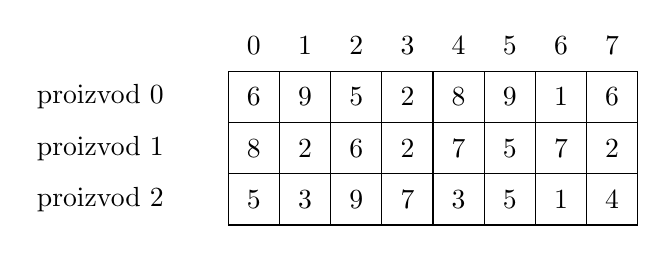
\begin{tikzpicture}[scale=.65]
    \draw (0, 0) grid (8,3);
    \node at (-2.5,2.5) {proizvod 0};
    \node at (-2.5,1.5) {proizvod 1};
    \node at (-2.5,0.5) {proizvod 2};

    \foreach \x in {0,...,7}
        {\node at (\x+0.5,3.5) {\x};}
    \foreach \x/\v in {0/6,1/9,2/5,3/2,4/8,5/9,6/1,7/6}
        {\node at (\x+0.5,2.5) {\v};}
    \foreach \x/\v in {0/8,1/2,2/6,3/2,4/7,5/5,6/7,7/2}
        {\node at (\x+0.5,1.5) {\v};}
    \foreach \x/\v in {0/5,1/3,2/9,3/7,4/3,5/5,6/1,7/4}
        {\node at (\x+0.5,0.5) {\v};}
\end{tikzpicture}
\end{center}
U ovom scenariju minimalna ukupna cijena je $5$:
\begin{center}
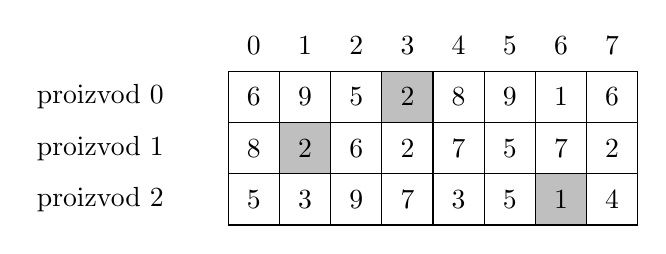
\begin{tikzpicture}[scale=.65]
    \fill [color=lightgray] (1, 1) rectangle (2, 2);
    \fill [color=lightgray] (3, 2) rectangle (4, 3);
    \fill [color=lightgray] (6, 0) rectangle (7, 1);
    \draw (0, 0) grid (8,3);
    \node at (-2.5,2.5) {proizvod 0};
    \node at (-2.5,1.5) {proizvod 1};
    \node at (-2.5,0.5) {proizvod 2};

    \foreach \x in {0,...,7}
        {\node at (\x+0.5,3.5) {\x};}
    \foreach \x/\v in {0/6,1/9,2/5,3/2,4/8,5/9,6/1,7/6}
        {\node at (\x+0.5,2.5) {\v};}
    \foreach \x/\v in {0/8,1/2,2/6,3/2,4/7,5/5,6/7,7/2}
        {\node at (\x+0.5,1.5) {\v};}
    \foreach \x/\v in {0/5,1/3,2/9,3/7,4/3,5/5,6/1,7/4}
        {\node at (\x+0.5,0.5) {\v};}
\end{tikzpicture}
\end{center}

Neka $\texttt{price}[x][d]$ označava cijenu proizvoda $x$
na dan $d$.
Na primjer, u gornjem scenariju $\texttt{price}[2][3] = 7$.
Zatim, neka $\texttt{total}(S,d)$ označava minimalnu ukupnu
cijenu kupnje podskupa $S$ proizvoda do dana $d$.
Pomoću te funkcije rješenje zadatka je
$\texttt{total}(\{0 \ldots k-1\},n-1)$.

Prvo, $\texttt{total}(\emptyset,d) = 0$,
jer kupnja praznog skupa ne košta ništa,
i $\texttt{total}(\{x\},0) = \texttt{price}[x][0]$,
jer postoji jedan način kupnje jednog proizvoda prvog dana.
Zatim se može koristiti sljedeća rekurzija:
\begin{equation*}
\begin{split}
\texttt{total}(S,d) = \min( & \texttt{total}(S,d-1), \\
& \min_{x \in S} (\texttt{total}(S \setminus x,d-1)+\texttt{price}[x][d]))
\end{split}
\end{equation*}
To znači da na dan $d$ ili ne kupujemo nijedan proizvod
ili kupujemo proizvod $x$ koji pripada skupu $S$.
U potonjem slučaju uklanjamo $x$ iz $S$ i dodajemo
cijenu proizvoda $x$ ukupnoj cijeni.

Sljedeći korak je izračunati vrijednosti funkcije
pomoću dinamičkog programiranja.
Za pohranu vrijednosti funkcije deklariramo niz
\begin{lstlisting}
int total[1<<K][N];
\end{lstlisting}
gdje su $K$ i $N$ dovoljno velike konstante.
Prva dimenzija niza odgovara bitovnom
zapisu podskupa.

Prvo, slučajevi u kojima je $d=0$ mogu se obraditi ovako:
\begin{lstlisting}
for (int x = 0; x < k; x++) {
    total[1<<x][0] = price[x][0];
}
\end{lstlisting}
Zatim se rekurzija prevodi u sljedeći kod:
\begin{lstlisting}
for (int d = 1; d < n; d++) {
    for (int s = 0; s < (1<<k); s++) {
        total[s][d] = total[s][d-1];
        for (int x = 0; x < k; x++) {
            if (s&(1<<x)) {
                total[s][d] = min(total[s][d],
                                    total[s^(1<<x)][d-1]+price[x][d]);
            }
        }
    }
}
\end{lstlisting}
Vremenska složenost algoritma je $O(n 2^k k)$.

\subsubsection{Od permutacija do podskupova}

Pomoću dinamičkog programiranja često je moguće
iteraciju po permutacijama zamijeniti
iteracijom po podskupovima\footnote{Ovu su tehniku 1962. godine uveli
M. Held i R. M. Karp \cite{hel62}.}.
Korist od toga je što je
$n!$, broj permutacija,
mnogo veći od $2^n$, broja podskupova.
Na primjer, ako je $n=20$, tada je
$n! \approx 2.4 \cdot 10^{18}$ i $2^n \approx 10^6$.
Stoga, za određene vrijednosti $n$,
možemo efikasno proći kroz podskupove, ali ne i kroz permutacije.

Kao primjer, razmotrimo sljedeći zadatak:
Postoji dizalo s maksimalnom težinom $x$,
i $n$ ljudi poznatih težina
koji žele doći s prizemlja
na najgornji kat.
Koliki je minimalan broj vožnji potreban
ako ljudi ulaze u dizalo u optimalnom redoslijedu?

Na primjer, pretpostavimo da je $x=10$, $n=5$
i da su težine sljedeće:
\begin{center}
\begin{tabular}{ll}
osoba & težina \\
\hline
0 & 2 \\
1 & 3 \\
2 & 3 \\
3 & 5 \\
4 & 6 \\
\end{tabular}
\end{center}
U ovom slučaju minimalan broj vožnji je 2.
Jedan optimalan redoslijed je $\{0,2,3,1,4\}$,
koji dijeli ljude u dvije vožnje:
prvo $\{0,2,3\}$ (ukupna težina 10),
a zatim $\{1,4\}$ (ukupna težina 9).

Zadatak se lako može riješiti u $O(n! n)$ vremenu
isprobavanjem svih mogućih permutacija $n$ ljudi.
Međutim, možemo koristiti dinamičko programiranje kako bismo dobili
efikasniji algoritam vremenske složenosti $O(2^n n)$.
Ideja je za svaki podskup ljudi izračunati
dvije vrijednosti: minimalan broj potrebnih vožnji i
minimalnu težinu ljudi koji se voze u posljednjoj grupi.

Neka $\texttt{weight}[p]$ označava težinu
osobe $p$.
Definiramo dvije funkcije:
$\texttt{rides}(S)$ je minimalan broj
vožnji za podskup $S$,
a $\texttt{last}(S)$ je minimalna težina
posljednje vožnje.
Na primjer, u gornjem scenariju
\[ \texttt{rides}(\{1,3,4\})=2 \hspace{10px} \textrm{i}
\hspace{10px} \texttt{last}(\{1,3,4\})=5,\]
jer su optimalne vožnje $\{1,4\}$ i $\{3\}$,
a druga vožnja ima težinu 5.
Naravno, naš je konačni cilj izračunati vrijednost
$\texttt{rides}(\{0 \ldots n-1\})$.

Vrijednosti funkcija možemo izračunati
rekurzivno i zatim primijeniti
dinamičko programiranje.
Ideja je proći kroz sve ljude
koji pripadaju skupu $S$ i optimalno
odabrati posljednju osobu $p$ koja ulazi u dizalo.
Svaki takav odabir daje podproblem
za manji podskup ljudi.
Ako je $\texttt{last}(S \setminus p)+\texttt{weight}[p] \le x$,
možemo dodati $p$ u posljednju vožnju.
Inače, moramo rezervirati novu vožnju
koja u početku sadrži samo $p$.

Za implementaciju dinamičkog programiranja
deklariramo niz
\begin{lstlisting}
pair<int,int> best[1<<N];
\end{lstlisting}
koji za svaki podskup $S$ sadrži
par $(\texttt{rides}(S),\texttt{last}(S))$.
Vrijednost za praznu grupu postavljamo ovako:
\begin{lstlisting}
best[0] = {1,0};
\end{lstlisting}
Zatim niz možemo popuniti na sljedeći način:

\begin{lstlisting}
for (int s = 1; s < (1<<n); s++) {
    // initial value: n+1 rides are needed
    best[s] = {n+1,0};
    for (int p = 0; p < n; p++) {
        if (s&(1<<p)) {
            auto option = best[s^(1<<p)];
            if (option.second+weight[p] <= x) {
                // add p to an existing ride
                option.second += weight[p];
            } else {
                // reserve a new ride for p
                option.first++;
                option.second = weight[p];
            }
            best[s] = min(best[s], option);
        }
    }
}
\end{lstlisting}
Uočimo da gornja petlja jamči da
za bilo koja dva podskupa $S_1$ i $S_2$
takva da je $S_1 \subset S_2$, obrađujemo $S_1$ prije $S_2$.
Stoga se vrijednosti dinamičkog programiranja izračunavaju u
ispravnom redoslijedu.

\subsubsection{Brojanje podskupova}

Naš posljednji zadatak u ovom poglavlju glasi:
Neka je $X=\{0 \ldots n-1\}$ i neka je svakom podskupu $S \subset X$
pridružen cijeli broj $\texttt{value}[S]$.
Naš je zadatak za svaki $S$ izračunati
\[\texttt{sum}(S) = \sum_{A \subset S} \texttt{value}[A],\]
tj. sumu vrijednosti podskupova skupa $S$.

Na primjer, pretpostavimo da je $n=3$ i da su vrijednosti sljedeće:
\begin{multicols}{2}
\begin{itemize}
\item $\texttt{value}[\emptyset] = 3$
\item $\texttt{value}[\{0\}] = 1$
\item $\texttt{value}[\{1\}] = 4$
\item $\texttt{value}[\{0,1\}] = 5$
\item $\texttt{value}[\{2\}] = 5$
\item $\texttt{value}[\{0,2\}] = 1$
\item $\texttt{value}[\{1,2\}] = 3$
\item $\texttt{value}[\{0,1,2\}] = 3$
\end{itemize}
\end{multicols}
U ovom slučaju, na primjer,
\begin{equation*}
\begin{split}
\texttt{sum}(\{0,2\}) &= \texttt{value}[\emptyset]+\texttt{value}[\{0\}]+\texttt{value}[\{2\}]+\texttt{value}[\{0,2\}] \\ 
                      &= 3 + 1 + 5 + 1 = 10.
\end{split}
\end{equation*}

Budući da ukupno postoji $2^n$ podskupova,
jedno moguće rješenje jest proći kroz sve
parove podskupova u $O(2^{2n})$ vremenu.
Međutim, pomoću dinamičkog programiranja
zadatak možemo riješiti u $O(2^n n)$ vremenu.
Ideja je usredotočiti se na sume u kojima su
elementi koji se smiju ukloniti iz $S$ ograničeni.

Neka $\texttt{partial}(S,k)$ označava sumu
vrijednosti podskupova skupa $S$ uz ograničenje
da se samo elementi $0 \ldots k$
smiju ukloniti iz $S$.
Na primjer,
\[\texttt{partial}(\{0,2\},1)=\texttt{value}[\{2\}]+\texttt{value}[\{0,2\}],\]
jer smijemo ukloniti samo elemente $0 \ldots 1$.
Vrijednosti funkcije \texttt{sum} možemo izračunati pomoću
vrijednosti funkcije \texttt{partial}, jer je
\[\texttt{sum}(S) = \texttt{partial}(S,n-1).\]
Bazni slučajevi za funkciju su
\[\texttt{partial}(S,-1)=\texttt{value}[S],\]
jer se u tom slučaju nijedan element ne može ukloniti iz $S$.
Zatim, u općem slučaju možemo koristiti sljedeću rekurziju:
\begin{equation*}
    \texttt{partial}(S,k) = \begin{cases}
               \texttt{partial}(S,k-1) & k \notin S \\
               \texttt{partial}(S,k-1) + \texttt{partial}(S \setminus \{k\},k-1) & k \in S
           \end{cases}
\end{equation*}
Ovdje se usredotočujemo na element $k$.
Ako je $k \in S$, imamo dvije mogućnosti: možemo ili zadržati $k$ u $S$
ili ga ukloniti iz $S$.

Postoji posebno domišljat način implementacije
izračuna suma. Možemo deklarirati niz
\begin{lstlisting}
int sum[1<<N];
\end{lstlisting}
koji će sadržavati sumu svakog podskupa.
Niz se inicijalizira ovako:
\begin{lstlisting}
for (int s = 0; s < (1<<n); s++) {
    sum[s] = value[s];
}
\end{lstlisting}
Zatim niz možemo popuniti na sljedeći način:
\begin{lstlisting}
for (int k = 0; k < n; k++) {
    for (int s = 0; s < (1<<n); s++) {
        if (s&(1<<k)) sum[s] += sum[s^(1<<k)];
    }
}
\end{lstlisting}
Ovaj kod izračunava vrijednosti $\texttt{partial}(S,k)$
za $k=0 \ldots n-1$ u niz \texttt{sum}.
Budući da se $\texttt{partial}(S,k)$ uvijek temelji na
$\texttt{partial}(S,k-1)$, možemo ponovno koristiti niz
\texttt{sum}, što daje vrlo efikasnu implementaciju.
